%************************************************
\chapter[Abstracting the robot]{Abstracting the robot}\label{ch:capabilities}
%************************************************

\begin{flushright}{\slshape The essence of abstractions is preserving information that is relevant in a given context, and forgetting information that is irrelevant in that context.} \\ \medskip
    ---  John V. Guttag
\end{flushright}

In the previous chapters we discussed extensively how to capture all the details of a robotic architecture, how to codify not only the topology of the components, but also their inner functionalities. We defined a collection of tools to help the \textit{system designer} and the \textit{component developer} in describing, designing, realising and implementing their vision. However, this is only the starting point of a process to modernise the development of software for robots, to make the creation of robotic applications as accessible as developing a mobile app, a web page or a video game.

The shortest path to make a technology more accessible is through abstraction. Robot software development has already benefited from this approach with the introduction of robotic middleware and frameworks, for example, the ROS computational graph creates an abstraction layer between the underlying hardware and the components. This made robotics more accessible and triggered a process that resulted in vast repositories of components efficiently implementing basic robot functionalities (\eg, navigation, perception, manipulation). 

However, the key element of abstraction is the context. Not every approach is useful to achieve a specific result. Technologies like ROS or other robotic middleware and frameworks are useful to streamline the development of components, but a different level of abstraction is needed to implement application at an higher level. Because of the success of component-based approaches, robotic system are becoming more complex and richer in functionalities attracting experts with diverse backgrounds that are more interested in the high-level capabilities expressed by the robot as as system, instead of focusing on the low-level functionalities implemented by each component.

These \textit{application developers} need a different type of abstraction that goes beyond the one provided by middleware and frameworks. In this chapter we tackle the problem of analysing the robot a system to capture the significant high-level functionalities and to create an abstraction that can be exploited to develop complex applications. First by defining an ontology that captures the structure of robot system, then using this framework to identify robot capabilities. These capabilities are the access point for creating an abstraction layer between a set of APIs and the underlying robot system. Lastly, we give an overview on how the model-based approach presented before can be used as a support for the concept of robot capabilities.

\minitoc
\newpage

\section{Ontology representation}
Creating new abstractions layers on top of an existing technology is not a difficult task, multiple approaches can be used: programming interfaces, libraries, frameworks, middleware, domain-specific languages, and more. For example programming interfaces usually remain in the same context of the abstracted technology and only provides controlled access to the underlying functionalities, their aim is to hide the complexity of the implementation, not to create a decoupling layer.  A similar overview can be done of libraries, they aggregate multiple simple functionalities in a single structured interface, but, again, the abstraction does not change the nature of the technology, it provides only a different way to interact with it. Frameworks push the abstraction a bit further, not only it hides the inner functioning of the system but provides entry points that a developer can use to extend the framework functionalities and create complex applications exploiting it. The aims of a middleware are similar: provide structure, give to developers basic functionalities, create an environment that can be used to implement application. However, the decoupling introduced between the developer and the underlying system is more significant (\eg, ROS supports both Python and C++ to implement the nodes). Domain-specific languages represent a more agnostic form of abstraction, since they present a completely different interface with respect to the target  technology, however, by definition, they are created with a narrow scope. In conclusion, most of these solutions have the downside of being focused vertically (\eg, programming interfaces and libraries) or horizontally (\eg, middleware and domain specific languages), since the abstraction they provide is usually created to target a specific category of user.

In an effort to achieve a more generalised abstraction from the underlying robot system, we decide to base our abstraction on an ontology. Ontologies have been successfully used to limit the complexity of the domain and to organise the information into data and knowledge.

\begin{figure}[t]
    \myfloatalign
    \subfloat[TODO]
    {\label{subfig:basic}%
    	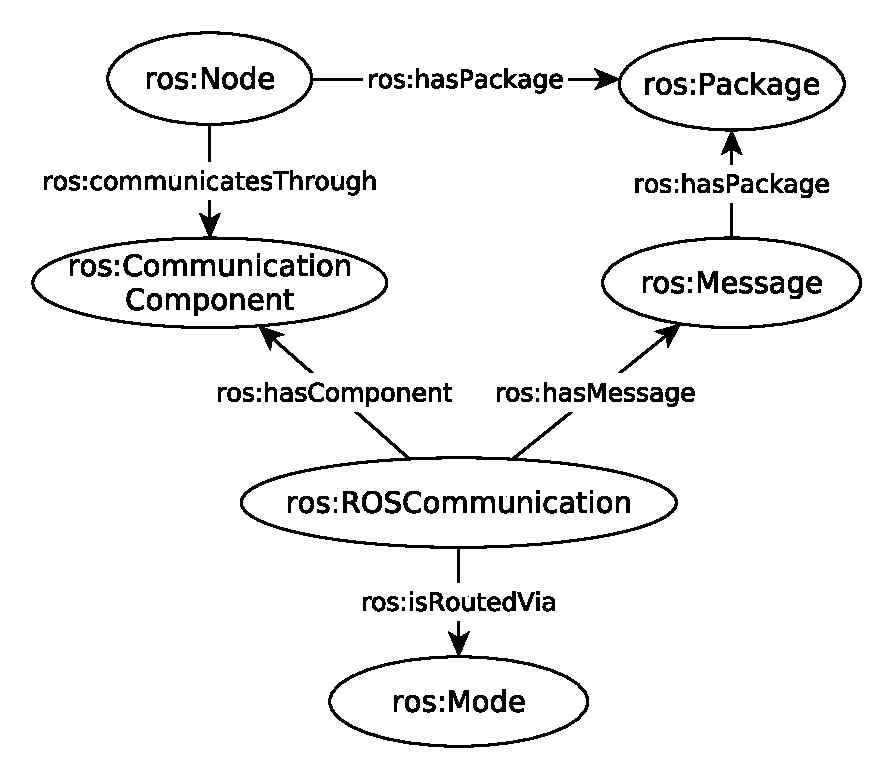
\includegraphics[width=.45\textwidth]{gfx/onto/basic}} 
    \subfloat[TODO]
    {\label{subfig:topic}%
    	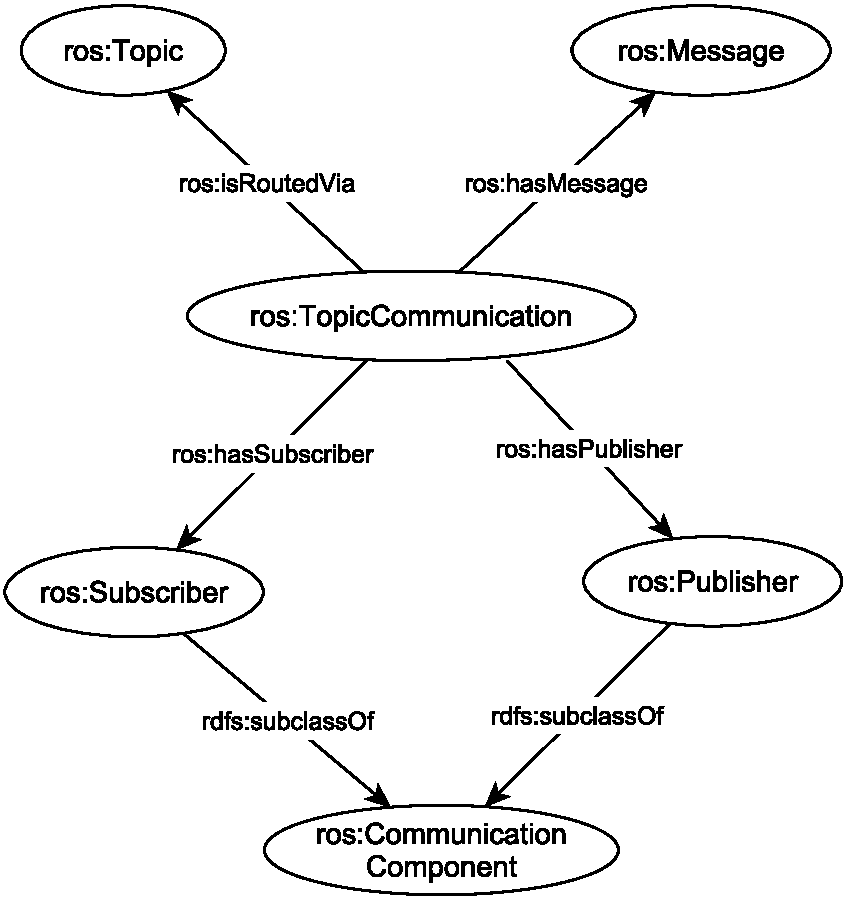
\includegraphics[width=.45\textwidth]{gfx/onto/topic}} \\
    \subfloat[TODO]
    {\label{subfig:service}%
    	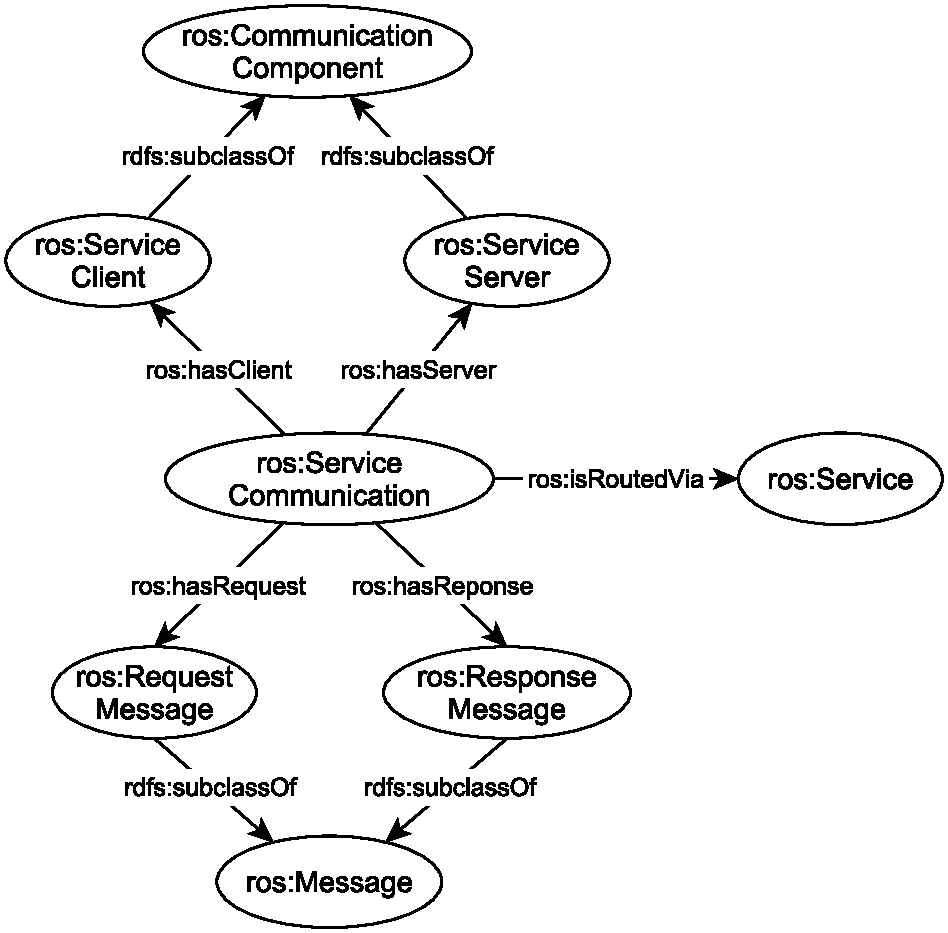
\includegraphics[width=.45\textwidth]{gfx/onto/service}}
    \caption[TODO]{TODO}\label{fig:ros-onto}
\end{figure}

\subsection{ROS description}
Before the definition of robot capabilities it is necessary to create a formal representation described as an ontology of the main elements of ROS. While this is not used directly in the capability extraction process, it creates a structure that can be used as a reference and to contextualise the capabilities. Since the aim is not the creation of an ontological classification of ROS, but to define a framework for capabilities classification and extraction, we did not capture in the ontology every element of ROS. 

The final aim is to automatically extract which capabilities are exposed by a specific system, therefore, we can only exploit static information provided by the source code or dynamic information obtained from the runtime of the system. Given that ROS support various runtime-only configuration (\eg, topic remapping, parameters definition at start-up, dynamic reconfigure, \etc), we decided to focus on all the information obtainable when the system is running. In ROS, during runtime, the main source of information comes from the computational graph, a collection of all the active nodes and their connections. Various elements, other than nodes, are part of the graph, for example the ROS master or the parameters server, to build our ontology, we decided to focus only on those parts that are defined by the developer, both as a topology definition and as a complete implementation. In particular, we take in account:
\begin{itemize}
\item A \textit{node} is a process performing a specific computation and represent the minimal executable unit of ROS. A single node or a collection of nodes implement a specific functionality, therefore is connected to a potential capability of the robot.
\item \textit{Messages} are the typed data structure exchanged by the nodes when communicating with each other. Here we refer to messages in the broader sense, including all communication object exchanged in any type of communication. Messages are often generic (\eg, \textit{Vector3} in the \textit{geometry\_msgs} package), but when specific (\eg, \textit{Image} in the package \textit{sensor\_msgs})  they can be used to identify capabilities.
\item \textit{Topics} are the named channels used to exchange messages asynchronously using a publish/subscribe paradigm. Since they are completely user-defined, it is not possible to infer any significant information from them, however, they are fundamental to categorise capability, especially if multiple instances of the same one are available (\eg, multiple vision systems).
\item Similarly to topics, \textit{services} are named channels for synchronous communication, exchanging pairs of messages (\ie, request and response). Again, the service itself does not provide significant information since it is user-defined, however, it helps categorise the identified capabilities.  
\end{itemize}
While they are an alternative communication system between nodes, actions are not included in this analysis for multiple reasons. First of all, they are rarely used, therefore any extra effort to include them would provide little or no extra information. Additionally, given their complexity, they are, in most cases, completely defined by the developer and not based on any pre-defined message. Lastly, from a pure communication point of view, actions are only a collection of topics with a specific set of rules hidden to the developer by the action clients. 

Focusing on these elements we can define a formal representation of ROS and the interactions of its components. As said before, the aim of this ontology is to support the definition of the concept of capabilities and their automatic extraction from an existing system, therefore, while it is based on the Event and Situation ontology design patterns, it is not rigorously designed for robustness, completeness or originality. Figure~\ref{fig:ros-onto} show a graphical representation of the ontology describing the main ROS elements (Figure~\ref{subfig:basic}), and a more detailed description of topics (Figure~\ref{subfig:topic}) and services (Figure~\ref{subfig:service}).

\paragraph{Basic ROS description} Figure~\ref{subfig:basic} capture the main elements of ROS and how they are conceptually interconnected. ROS revolves around the concept of the computational graph, where nodes (\ie, executable components) are connected to each other through different type of communications (\ie, topics and services). Messages are the main carrier of information between different components. In ROS, there is one way to loosely aggregate elements by functionalities: packages. Nodes and messages have an assigned package, which is user defined, therefore not all of them are a reliable source of information to define the expected functionalities of an element. Nevertheless, some effort to create standard packages exists, some examples are \textit{sensor\_msgs} for messages used to encode sensor measurements, or \textit{navigation} for the planning, mapping and control nodes.

All these details are codified by the ontology. \textit{ros:Node} and \textit{ros:Message} are defined as part of a specific \textit{ros:Package}. The edges of the computational graph are identified by the \textit{ros:ROS\-Com\-mu\-ni\-ca\-tion} class, multiple relations exists between this class and the rest of the ontology. To identify the type of communication, we use the \textit{ros:Mode} class and the relation \textit{ros:isRoutedVia}, together they specify if a pair of nodes use an asynchronous (\ie, topic-based) or synchronous (\ie, service-based) communication system. The relation between \textit{ros:Node} and \textit{ros:ROS\-Com\-mu\-ni\-ca\-tion} is not direct, but it is mediated by a \textit{ros:Communication Component}. This class represent the interface implemented by the node to use a specific communication pattern, moreover, it is important to define the direction of the communication. For example, the a velocity message published by a single node and read by a multitude is more probably related by a speedometer, while multiple velocity publisher converging on a single subscriber can point to a set-point multiplexer.

This ontology was defined independently from the modelling approach defined in Chapter~\ref{ch:Modelling} and with no intention of establishing a encompassing definition. Nevertheless, there are recurring structures that appear both in the ontology and the  model. Clearly some are related to the internal structure of robotic middleware and frameworks, or mode in details to ROS itself. For example the definition of nodes (\ie, robotic components in the \textit{component-and-connector paradigm}) and messages (\ie, communication objects) appears in most component-based approaches. However, the necessity of specify a communication component acting as an interface between the the node and the communication system, is the same as the need to define AADL threads as a way to model the inner functioning of a component. In summary, it is never enough to just specify a components and its connection, it is necessary to detail the communication, its direction, the protocol, and the management system.

\paragraph{Topic description} Figure~\ref{subfig:topic} represents the extension of the previous ontology to better describe communication happening through topics. The central class of this ontology is \textit{ros:Topic\-Com\-mu\-ni\-ca\-tion}, which is a subclass of the more general \textit{ros:ROS\-Com\-mu\-ni\-ca\-tion}. Here we specify more in detail the protocol used by this type of communication by creating a subclass of \textit{ros:Mode} and defining \textit{ros:Topic}. The topic-based communication is the simplest protocol provided by ROS, implementing an asynchronous interaction based on the publish/subscribe protocol, additionally it uses a publish-and-forget approach. This is translated in the ontology by defining two subclasses for the communication component: \textit{ros:Subscriber}, as the subscriber of the protocol, in charge of receiving the messages, and \textit{ros:Publisher}, as the publisher, in charge of generating the messages. The lack of ownership of the messages and the absence of delivery confirmation result in a simple relation between the message and the topic.

To understand how an instance of a topic is defined with respect to the corresponding nodes, we  can take as an example a simple pair of nodes implementing a local planner feeding a control system with velocity set-points. They are connected by a named topic (\texttt{/cmd\_vel}) and exchange a specific type of message (\textit{geometry\_msgs/Twist}). The local planner implements a publisher, while the control system implements a subscriber. The resulting representation is in Listing~\ref{lst:onto-topic}.

\begin{lstlisting}[frame=tb,caption={TODO},label=lst:onto-topic]
@prefix ros: <onto-ros/class#>
@prefix : <onto-ros/resource/>
:setpoints a ros:TopicCommunication;
	ros:isRoutedVia :cmd_vel;
	ros:hasMessage :twist;
	ros:hasPublisher :cmd-output;
	ros:hasSubscriber :cmd-input.
:twist a ros:Message.
:cmd-vel a ros:Topic.  
:local-planner a ros:Node;
	ros:hasComponent :cmd-output.
:controller a ros:Node;
	ros:hasComponent :cmd-input.
 \end{lstlisting}

\paragraph{Service description} Figure~\ref{subfig:service} represent a second extension of the basic ontology to describe the synchronous communication approach provided by services.  As for topics, the central class is \textit{ros:Service\-Com\-mu\-ni\-ca\-tion} as a subclass of \textit{ros:ROS\-Com\-mu\-ni\-ca\-tion}. To identify the protocol implemented by services, we created a dedicated subclass of \textit{ros:Mode} called \textit{ros:Service}. Given their
synchronous approach, messages exchanged during the execution of a service are divided in two categories: requests, sent by the client to trigger the functionality provided by the service, and response, sent by the server with the result of the computation or as a completion notification. To capture this we defined two subclasses of the original \textit{ros:Message}: \textit{ros:Request Message} used to classify the request sent by the client, and \textit{ros:Response Message} used to identify the response sent by the server. As for the topic, it is necessary to specify, using subclasses of \textit{ros:Communication Component}, the specific interfaces implemented by the node when acting as a client or as a server. The two subclasses are: \textit{ros:Service Client}, for the client interface, and \textit{ros:Service Server}, for the server interface.

Listing~\ref{lst:onto-service} provides a small example on how an instance of a service is represented using the ontology. In the example there is a global planner that needs to synchronously request an occupancy grid from the map server. They interact using a named channel (\texttt{/map}), the client (\ie, the global planner) send an empty message (\textit{std\_msgs/Empty}) as a request to the server (\ie, the map server) to trigger the delivery of the map through the response (\textit{nav\_msgs/OccupancyGrid}). Each node, depending on its role, implements a service client or a service server.

\begin{lstlisting}[frame=tb,caption={TODO},label=lst:onto-service]
@prefix ros: <onto-ros/class#>
@prefix : <onto-ros/resource/>
:map-service a ros:ServiceCommunication;
       ros:isRoutedVia :map;
       ros:hasMessage :occupancy-grid;
       ros:hasClient :map-request;
       ros:hasServer :map-response.
:occupancy-grid a ros:Message.
:map a ros:Service.  
:global-planner a ros:Node;
       ros:hasComponent :map-request.
:map-server a ros:Node;
       ros:hasComponent :map-response.
 \end{lstlisting}



\subsection{Capabilities extraction}
\lipsum[2-4]

\section{Robot APIs} 
\lipsum[2-4]

\subsection{Local python interface}
\lipsum[2-4]

\subsection{Remote python interface} 
\lipsum[2-4]

\subsection{Web interface}
\lipsum[2-4]

\section{Bridge models and capabilities}

\subsection{Automatic functionality checker}

\subsection{Automatic architecture builder}
%*****************************************
